\documentclass[11pt,letterpaper]{article}

\usepackage[utf8]{inputenc}
\usepackage[T1]{fontenc}
\usepackage[spanish,es-nodecimaldot,es-tabla]{babel}
\usepackage{amsmath}
\usepackage{amssymb}
\usepackage{booktabs}
\usepackage{float}
\usepackage{graphicx}
\usepackage{caption}
\usepackage{subcaption}
% Las subfiguras también se listan en el índice de figuras.
\captionsetup[subfigure]{list=true}
\usepackage[hidelinks]{hyperref}
\usepackage[margin=1in]{geometry}

\graphicspath{{../../results/figures/}}

\title{Trabajo práctico 2: Detección de spam con aprendizaje supervisado y no supervisado}
\author{Alejandro Quesada \and Jose Herrera \and Manfred Azofeifa}
\date{\today}

\begin{document}

\maketitle
\tableofcontents
\newpage
\listoffigures
\newpage

% Una sección por punto del enunciado: cada responsable edita solo su archivo.
\section{Introducción}

Este informe documenta el Trabajo práctico 2 del curso de Principios de
Inteligencia Artificial. El trabajo consiste en detectar mensajes spam del
dataset SMSSpamCollection \cite{almeida2011sms,uci_sms_spam}, un conjunto
público de mensajes SMS etiquetados como \emph{ham} o \emph{spam}, con tres
enfoques implementados en PyTorch \cite{paszke2019pytorch}:

\begin{enumerate}
    \item clasificación supervisada con regresión logística sobre las
    características de un codificador, con y sin reducción de
    dimensionalidad por análisis de componentes principales;
    \item detección de anomalías con densidades por histograma y un umbral
    de verosimilitud;
    \item clasificación con modelos grandes de lenguaje.
\end{enumerate}

La implementación completa está en el notebook
\texttt{tp2\_detector\_spam.ipynb}, organizado en celdas de definiciones,
configuración, experimentos y análisis. Las pruebas unitarias, entregadas
en la carpeta \texttt{tests/} junto al notebook, cargan las mismas
definiciones sin ejecutar descargas ni experimentos. Las métricas, figuras y
tablas de este informe provienen de la ejecución de las secciones del
notebook. El punto 3 evalúa una línea base sin ajuste (3.1), dos modelos
adicionales con cuantización NF4 (3.2) y el ajuste de Qwen 14B con LoRA en
una partición fija (3.3), que eleva el F1 de 0.7120 a 0.9708 en su prueba
reservada.

\subsection{Protocolo común}

\begin{itemize}
    \item \textbf{Etiquetas.} \emph{ham} $=0$ y \emph{spam} $=1$; spam es la
    clase positiva del F1-score y la anomalía del detector.
    \item \textbf{Métricas.} Tasa de aciertos y F1-score.
    \item \textbf{Particiones.} 30 particiones estratificadas de 70~\% de
    entrenamiento y 30~\% de prueba, una por semilla.
    \item \textbf{Muestreo de los modelos de lenguaje.} 30 muestras
    estratificadas del 30~\% del dataset.
    \item \textbf{Codificador.} \texttt{sentence-transformers/all-mpnet-base-v2},
    con vectores de 768 dimensiones (Sección~\ref{sec:caracteristicas}).
    \item \textbf{Hiperparámetros de la regresión logística.} Calibrados por
    F1 en una validación interna de cada corrida, tomada solo de su entrenamiento
    (Sección~\ref{sec:calibracion}).
    \item \textbf{Dimensión óptima del PCA.} Se eligió $D=384$ para la
    regresión logística, la mitad de las 768 características
    (Sección~\ref{sec:pca}).
    \item \textbf{Detector de anomalías.} Entre los casos de 1.5, el detector
    de histogramas usa $D=2$, elegida en una validación interna de los 30
    entrenamientos; las densidades se construyen solo con ham y el umbral es
    el cuantil 5~\% de un 20~\% de ham reservado (Sección~\ref{sec:punto2}).
    Esta variante difiere de reutilizar $D=384$, como pide la lectura literal
    del apartado 2.1; por eso también se informa el detector con $D=384$.
    \item Punto 3.1: \texttt{Qwen/Qwen2.5-3B-Instruct}, prompt sin ejemplos
    en inglés y decodificación voraz; las respuestas ambiguas cuentan como
    ham. Las 30 muestras estratificadas del 30~\% usan las semillas de los
    puntos 1 y 2 (Sección~\ref{sec:punto3}). Para 3.2 se usan
    Mistral-7B-Instruct-v0.3 y Qwen2.5-14B-Instruct, ambos con NF4 de 4 bits
    y cálculo bfloat16. En 3.3 se ajusta Qwen 14B con LoRA sobre NF4, con un
    entrenamiento y una prueba reservada (Sección~\ref{sec:punto33}).
\end{itemize}

\section{Aprendizaje supervisado: regresión logística}
\label{sec:punto1}

% Punto 1 (60 puntos). Archivo: src/tp2/punto1.py. Pruebas: tests/test_punto1.py.

\subsection{Evaluación del modelo}

La regresión logística modela la probabilidad de que un mensaje sea spam como
\[
    p(y=1\mid x) = \sigma(x^\top w + b), \qquad \sigma(z) = \frac{1}{1+e^{-z}}.
\]
La función \texttt{forward} es una implementación propia en PyTorch
\cite{paszke2019pytorch}, sin \texttt{torch.nn}. Calcula los logits
$z = Xw + b$ de las $n$ muestras con un único producto matriz-vector y les
aplica la sigmoide. Para que la sigmoide no se desborde con logits grandes,
se evalúa con $e^{-|z|}\in(0,1]$:
\[
    \sigma(z) =
    \begin{cases}
        \dfrac{1}{1+e^{-|z|}} & z \geq 0,\\[2ex]
        \dfrac{e^{-|z|}}{1+e^{-|z|}} & z < 0.
    \end{cases}
\]
Ninguna de las dos ramas produce infinitos, ni en el valor ni en el
gradiente, mientras que la forma directa $1/(1+e^{-z})$ calcula $e^{1000}$
para $z=-1000$ y su gradiente con Autograd resulta indefinido.

\subsection{Entrenamiento}

La función \texttt{train\_logistic\_regression} minimiza la entropía cruzada
binaria media
\[
    L(w,b) = -\frac{1}{n}\sum_{i=1}^{n}
    \left[y_i\log p_i + (1-y_i)\log(1-p_i)\right],
    \qquad p_i = \sigma(x_i^\top w + b),
\]
con descenso del gradiente por lotes completos, también implementado sin
optimizadores de PyTorch. En cada época se evalúa $p$ con \texttt{forward} y
se aplica el gradiente exacto de $L$:
\[
    w \leftarrow w - \frac{\alpha}{n} X^\top (p - y), \qquad
    b \leftarrow b - \frac{\alpha}{n} \sum_{i=1}^{n} (p_i - y_i).
\]
Los pesos se inicializan con una normal de desviación $0.01$ generada con la
semilla de la corrida y el sesgo, en cero, de modo que la misma semilla
reproduce el mismo modelo. El entrenamiento ejecuta un número fijo de épocas
con una tasa de aprendizaje $\alpha$ fija: $\alpha=0.1$ y 1000 épocas en los
datos sintéticos, y $\alpha=10$ y 2000 épocas, calibrados en la
Sección~\ref{sec:calibracion}, sobre los mensajes. El historial de pérdida
guarda la pérdida inicial y la de cada época, calculada como
$\log(1+e^{z_i}) - y_i z_i$, expresión equivalente a la entropía cruzada que
no se indefine cuando $p_i$ vale exactamente 0 o 1.

\subsection{Verificación con datos linealmente separables}
\label{sec:sinteticos}

Antes de usar los mensajes, se verifica el regresor en un caso donde la
respuesta correcta se conoce. La frontera verdadera es la recta
\[
    w^{*\top}x + b^* = 0.6\,x_1 + 0.8\,x_2 - 0.5 = 0 .
\]
Como $\lVert w^*\rVert = 1$, $w^{*\top}x+b^*$ es la distancia con signo de
$x$ a la recta. Cada punto se coloca a una distancia
$|d| = 1 + 0.5\,|z|$, con $z\sim\mathcal{N}(0,1)$, del lado de su clase (la
clase 1 donde $d>0$) y a una posición $\mathcal{N}(0, 2^2)$ a lo largo de la
recta. Entre las dos clases queda una franja vacía de ancho 2, así que los
datos son linealmente separables por construcción. Se generan 200 puntos de
entrenamiento (100 por clase) y otros 200 de prueba con otra semilla
(Figura~\ref{fig:sinteticos-datos}).

\begin{figure}[H]
    \centering
    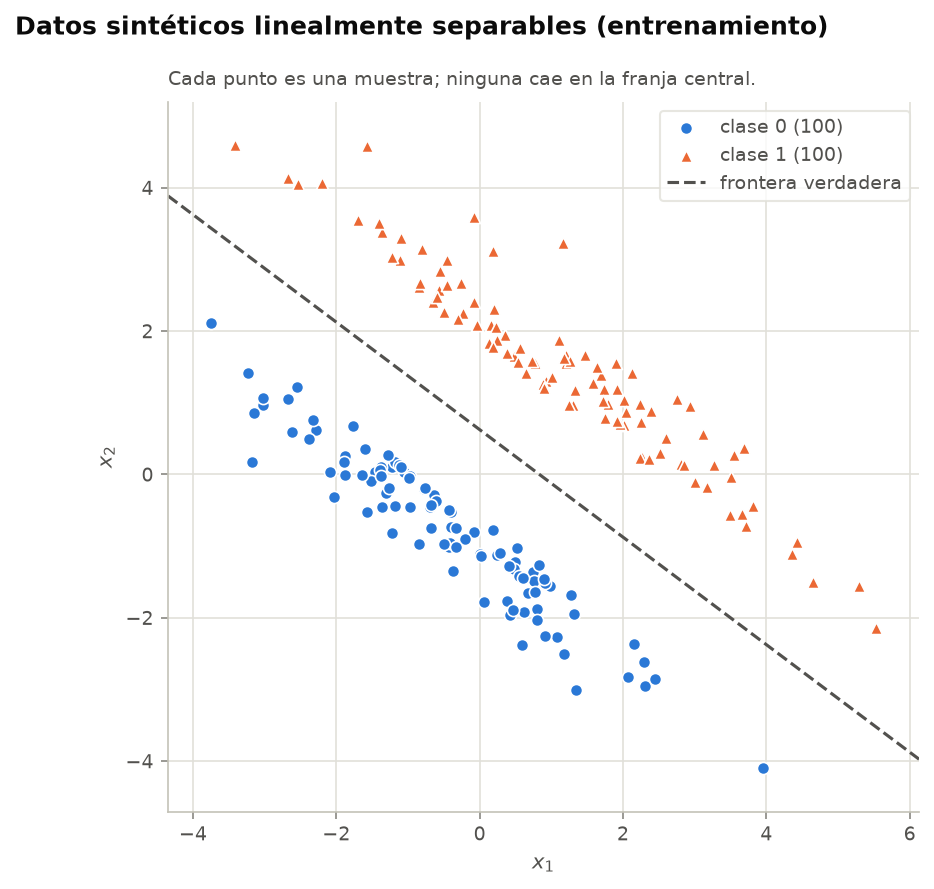
\includegraphics[width=0.62\textwidth]{datos-sinteticos-linealmente-separables-entrenamiento}
    \caption{Datos sintéticos de entrenamiento y frontera verdadera.}
    \label{fig:sinteticos-datos}
\end{figure}

El modelo se entrena con $\alpha=0.1$ durante 1000 épocas. Como el
entrenamiento es determinista para una semilla dada, entrenar $k$ épocas
reproduce exactamente el estado del entrenamiento completo en la época $k$;
así se obtienen las fronteras intermedias de la
Figura~\ref{fig:sinteticos-proceso}. La Tabla~\ref{tab:sinteticos-evolucion}
compara cada estado con la frontera verdadera: como la recta $w^\top x+b=0$
no cambia al multiplicar $w$ y $b$ por una constante, se reportan $w$ y $b$
divididos por $\lVert w\rVert$ y el ángulo entre $w$ y $w^*$.

\begin{figure}[H]
    \centering
    \begin{subfigure}{0.49\textwidth}
        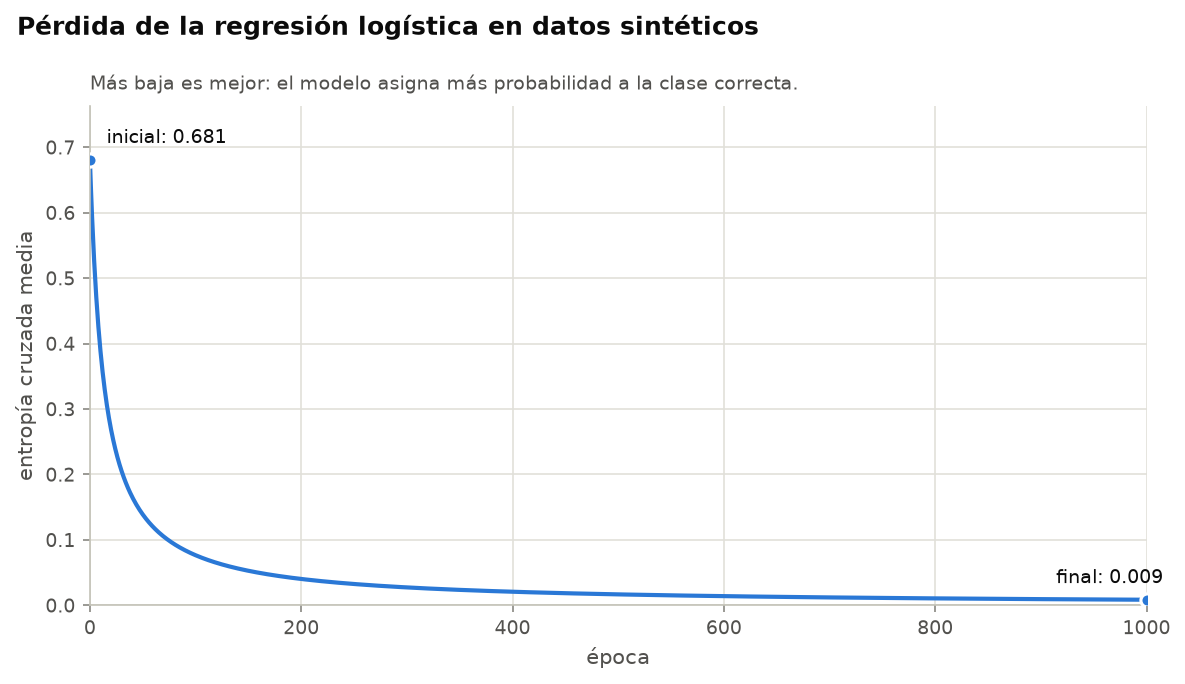
\includegraphics[width=\linewidth]{perdida-de-la-regresion-logistica-en-datos-sinteticos}
        \caption{Entropía cruzada media en cada época.}
    \end{subfigure}
    \hfill
    \begin{subfigure}{0.49\textwidth}
        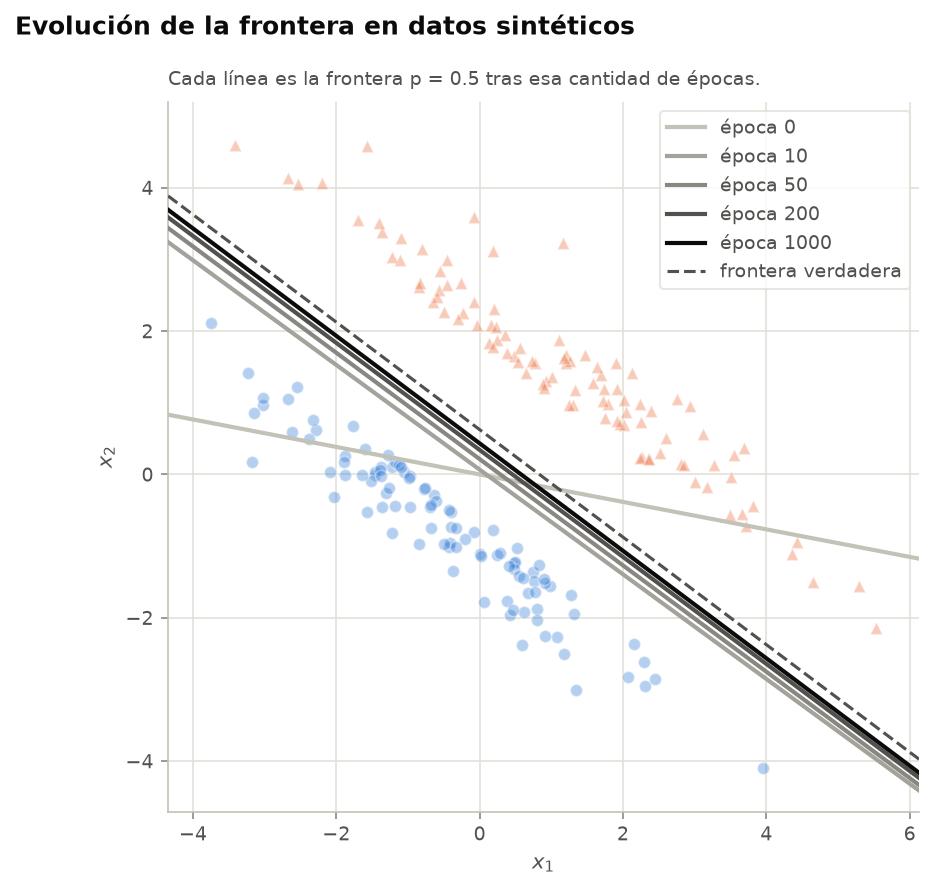
\includegraphics[width=\linewidth]{evolucion-de-la-frontera-en-datos-sinteticos}
        \caption{Frontera $p=0.5$ tras 0, 10, 50, 200 y 1000 épocas.}
    \end{subfigure}
    \caption{Proceso de entrenamiento sobre los datos sintéticos.}
    \label{fig:sinteticos-proceso}
\end{figure}

\begin{table}[H]
    \centering
    \caption{Evolución del entrenamiento en datos sintéticos.}
    \label{tab:sinteticos-evolucion}
    \small
    \begin{tabular}{rcccccc}
        \toprule
        Época & Pérdida & Aciertos (entr.) & $w_1/\lVert w\rVert$ & $w_2/\lVert w\rVert$ & $b/\lVert w\rVert$ & Ángulo con $w^*$ \\
        \midrule
        0    & 0.681 & 0.90 & 0.188 & 0.982 & 0.000  & 26.02° \\
        10   & 0.388 & 1.00 & 0.590 & 0.808 & $-0.054$ & 0.73° \\
        50   & 0.139 & 1.00 & 0.596 & 0.803 & $-0.172$ & 0.31° \\
        200  & 0.040 & 1.00 & 0.598 & 0.801 & $-0.274$ & 0.13° \\
        1000 & 0.009 & 1.00 & 0.600 & 0.800 & $-0.347$ & 0.01° \\
        \midrule
        Verdadera & --- & --- & 0.600 & 0.800 & $-0.500$ & 0° \\
        \bottomrule
    \end{tabular}
\end{table}

\begin{figure}[H]
    \centering
    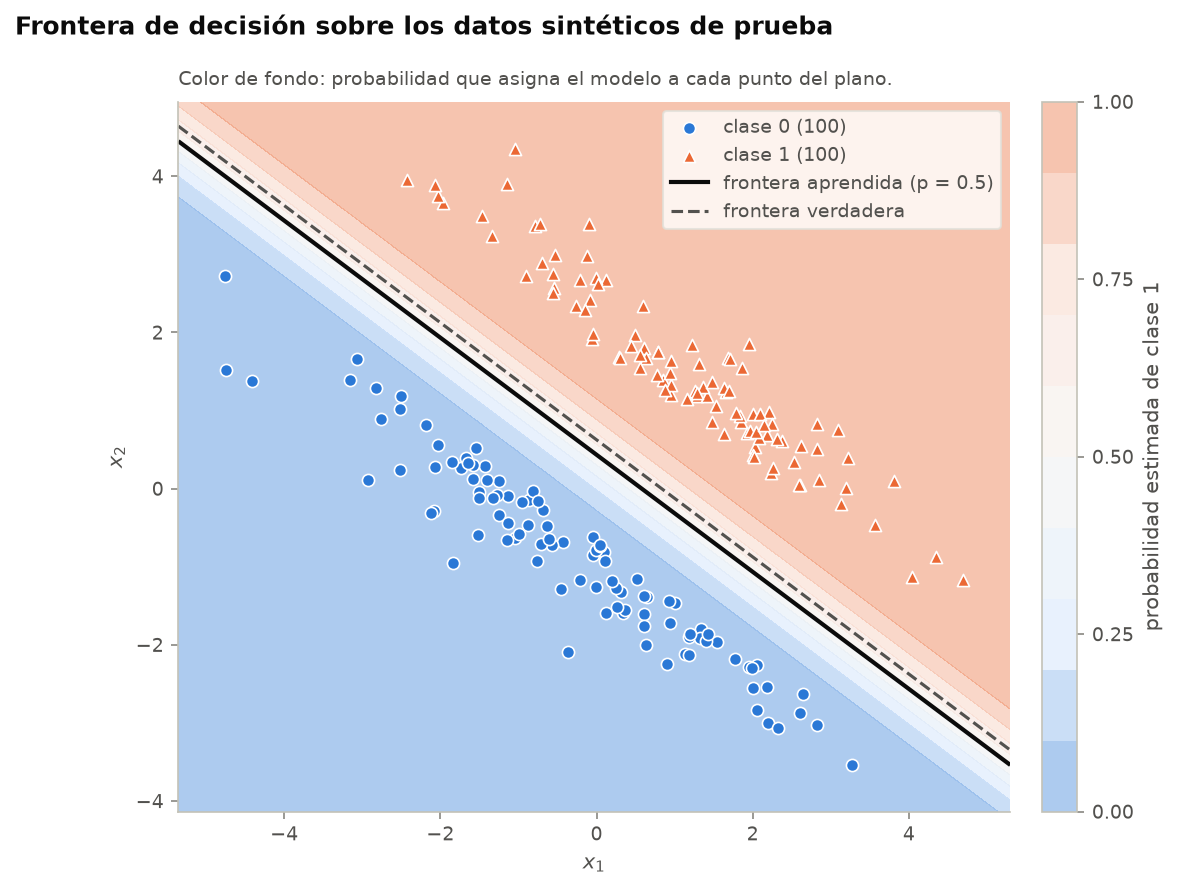
\includegraphics[width=0.7\textwidth]{frontera-de-decision-sobre-los-datos-sinteticos-de-prueba}
    \caption{Probabilidad estimada por el modelo final y frontera aprendida
    sobre los 200 puntos de prueba.}
    \label{fig:sinteticos-frontera}
\end{figure}

El regresor recupera la frontera verdadera. En la época 0 los pesos son casi
nulos ($\lVert w\rVert=0.02$) y la frontera está girada 26° respecto de la
verdadera; tras 10 épocas ya clasifica bien todo el entrenamiento y tras 1000
el ángulo es de 0.01°. La pérdida baja de 0.681 a 0.009 sin oscilar. En los
200 puntos de prueba la tasa de aciertos y el F1-score valen 1
(Figura~\ref{fig:sinteticos-frontera}).

Dos detalles muestran cómo aprende la regresión logística con datos
separables. Primero, $\lVert w\rVert$ crece sin parar (de 0.02 a 3.84): como
existe una recta que separa todo, la pérdida se puede seguir reduciendo
haciendo más abrupta la transición de probabilidad, sin cambiar la recta; por
eso la franja de colores alrededor de la frontera es angosta. Segundo, el
sesgo normalizado ($-0.35$) todavía no alcanza el verdadero ($-0.5$): la
frontera aprendida está desplazada 0.15 hacia la clase 0, pero dentro de la
franja vacía, así que clasifica todo bien. Con datos separables hay infinitas
rectas que separan perfectamente, y el descenso del gradiente se mueve muy
lentamente hacia la de margen máximo \cite{soudry2018implicit}: la
orientación converge mucho antes que la posición.

\subsection{Extracción de características y clasificación}
\label{sec:caracteristicas}

\paragraph{Codificador.} Cada mensaje, sin preprocesar, se convierte en un
vector con \texttt{all-MiniLM-L6-v2}, un modelo de la biblioteca
sentence-transformers \cite{reimers2019sentence} basado en MiniLM
\cite{wang2020minilm} y entrenado para que oraciones de significado parecido
queden cerca. Produce vectores de $D=384$ dimensiones con norma 1. Se eligió
frente a BERT base y DistilBERT porque está pensado para representar
oraciones completas y codifica los 5\,574 mensajes en CPU en poco tiempo. Las
características se calculan una sola vez y se guardan, porque no dependen de
la partición.

\paragraph{Calibración.}
\label{sec:calibracion}
Con vectores de norma 1, cada coordenada vale del orden de
$1/\sqrt{384}\approx0.05$ y el gradiente es pequeño: con $\alpha=0.1$ y
1000 épocas, los valores de la Sección~\ref{sec:sinteticos}, el modelo casi
no aprende (en una ejecución preliminar, el F1 medio de las 30 corridas fue
0.23). Para elegir $\alpha$ y las épocas sin usar la prueba, se tomó el
70~\% de entrenamiento de la primera partición y se separó de él un 20~\%
estratificado como validación (781 mensajes, 105 de ellos spam). Con el 80~\%
restante se entrenó cada combinación de
$\alpha\in\{0.5,1,2,5,10,20,50\}$ y $\{250,500,1000,2000,4000\}$ épocas, y
se eligió la de mayor F1 en la validación. Como el F1 de una validación con
105 spam cambia a saltos, varias combinaciones empatan; el empate se resolvió
con la menor entropía cruzada en la validación
(Figura~\ref{fig:calibracion}).

\begin{figure}[H]
    \centering
    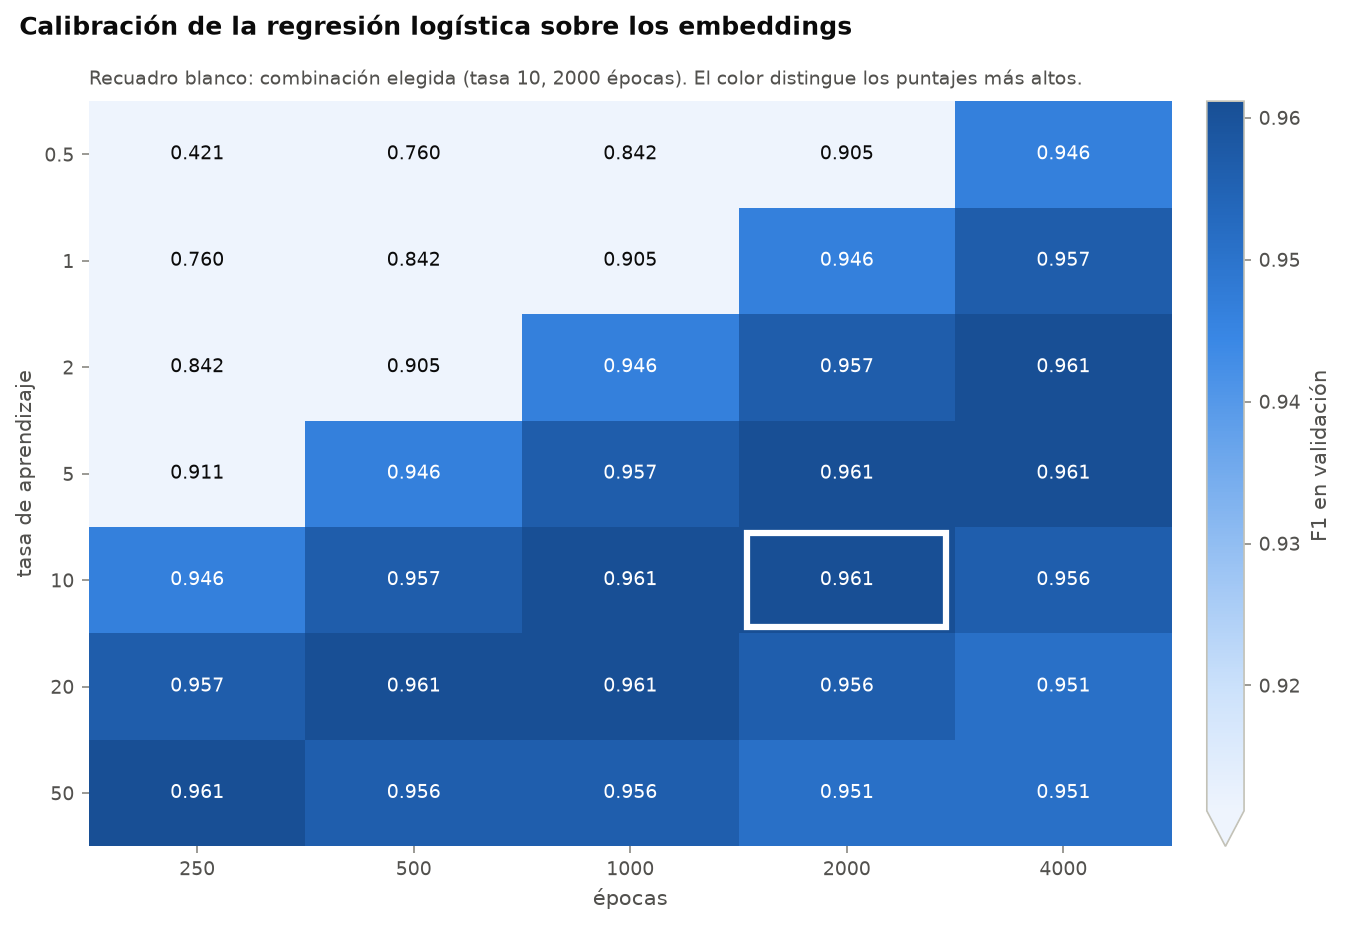
\includegraphics[width=0.85\textwidth]{calibracion-de-la-regresion-logistica-sobre-los-embeddings}
    \caption{F1 en la validación para cada combinación de tasa de
    aprendizaje y épocas.}
    \label{fig:calibracion}
\end{figure}

Lo que importa es el producto $\alpha\times$épocas: $10\times2000$,
$5\times4000$ y $20\times1000$ (todas 20\,000) dan el mismo F1 de validación
(0.961) y casi la misma pérdida (0.0463). Con poco entrenamiento el F1 cae a
0.42 ($0.5\times250$); con demasiado ($50\times4000$) la pérdida de ajuste
sigue bajando (0.004), pero la de validación sube (0.059) y el F1 baja a
0.951, una señal leve de sobreajuste. Se eligieron $\alpha=10$ y 2000 épocas.

\paragraph{Resultados de las 30 corridas.} Cada corrida usa una partición
estratificada 70/30 distinta, entrena con los valores calibrados y evalúa en
su prueba de 1\,672 mensajes (1\,448 ham y 224 spam). La
Tabla~\ref{tab:resultados-rl} resume las métricas y la
Figura~\ref{fig:resultados-rl} muestra cada corrida y la matriz de confusión
promedio.

\begin{table}[H]
    \centering
    \caption{Regresión logística sobre las características del codificador
    (30 corridas).}
    \label{tab:resultados-rl}
    \begin{tabular}{lcccc}
        \toprule
        Métrica & Media & Desviación & Mínimo & Máximo \\
        \midrule
        Tasa de aciertos & 0.9876 & 0.0022 & 0.9839 & 0.9916 \\
        F1-score         & 0.9528 & 0.0084 & 0.9388 & 0.9683 \\
        \bottomrule
    \end{tabular}
\end{table}

\begin{figure}[H]
    \centering
    \begin{subfigure}{0.52\textwidth}
        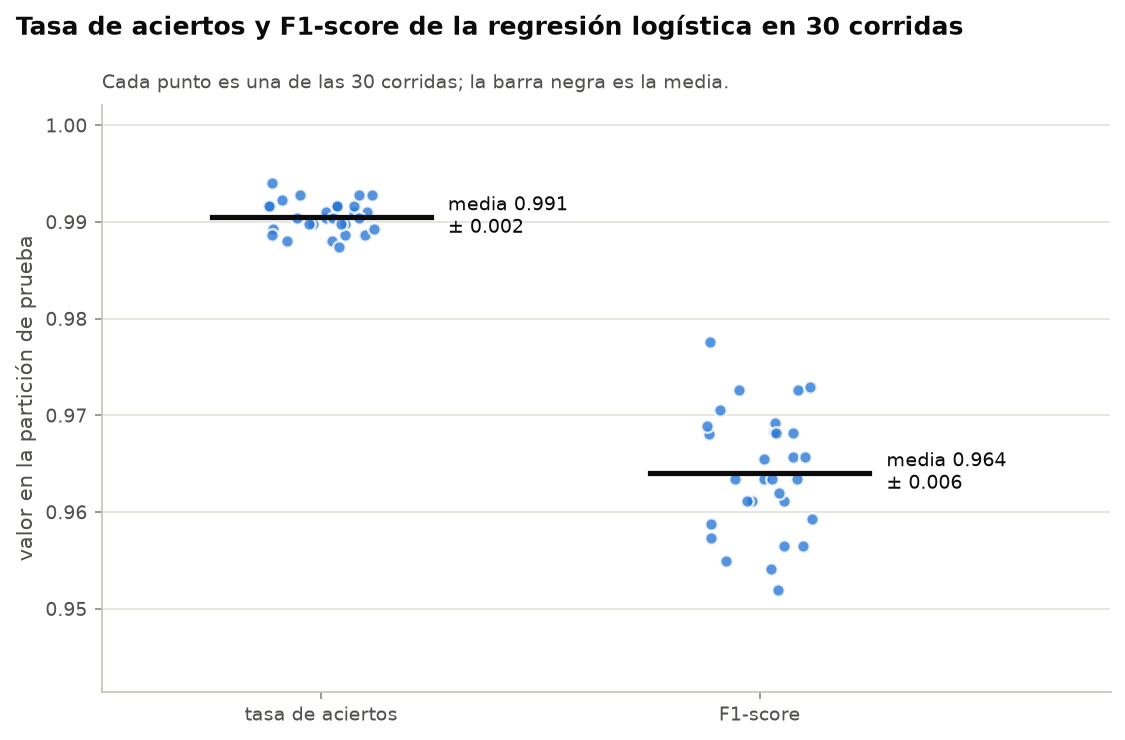
\includegraphics[width=\linewidth]{tasa-de-aciertos-y-f1-score-de-la-regresion-logistica-en-30-corridas}
        \caption{Métricas de cada corrida y su media.}
    \end{subfigure}
    \hfill
    \begin{subfigure}{0.44\textwidth}
        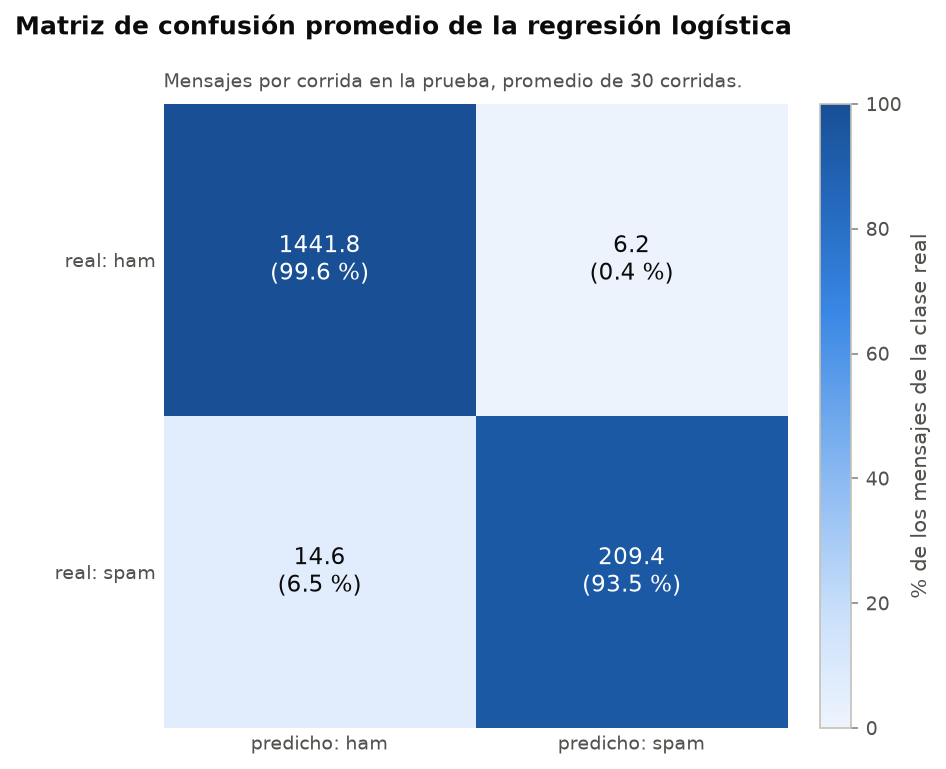
\includegraphics[width=\linewidth]{matriz-de-confusion-promedio-de-la-regresion-logistica}
        \caption{Matriz de confusión promedio.}
    \end{subfigure}
    \caption{Resultados de la regresión logística en las 30 corridas.}
    \label{fig:resultados-rl}
\end{figure}

La dispersión entre corridas es pequeña, así que el resultado no depende de
una partición afortunada. El F1 varía más que la tasa de aciertos porque solo
depende de los 224 spam de cada prueba: cada spam mal clasificado lo mueve
unas 0.0025. En promedio, de los 1\,448 ham solo 6.2 se marcan como spam
(0.4~\%), mientras que de los 224 spam se escapan 14.6 (6.5~\%): precisión
0.971 y exhaustividad 0.935. Casi todos los errores son spam que el modelo
deja pasar, el lado preferible para un filtro, porque perder un mensaje real
es peor que recibir un spam; bajar el umbral de 0.5 detectaría más spam a
costa de más falsas alarmas. Como referencia, un clasificador que respondiera
siempre ``ham'' tendría una tasa de aciertos de 0.866 y un F1 de 0.

Una limitación: la calibración usa datos de la primera partición que en otras
corridas pueden caer en la prueba. Solo se eligieron dos números con ellos,
así que el sesgo optimista es pequeño, pero existe.

\subsection{Reducción de dimensionalidad con PCA}

TODO (punto 1.5): describir el PCA, graficar el dataset reducido a 50~\%,
25~\% y 2 dimensiones, analizar la clasificación con regresión logística en
cada caso y justificar la $D$ óptima que usa el detector de anomalías.

\section{Detección de anomalías: umbral de verosimilitud}
\label{sec:punto2}

% Punto 2 (30 puntos). Archivo: src/tp2/punto2.py. Pruebas: tests/test_punto2.py.

\subsection{Densidades por histograma}

TODO (punto 2.1): describir la estimación de $p_1,\dots,p_D$, graficar y
comentar las densidades, y definir el umbral sobre la suma de
verosimilitudes.

\subsection{Evaluación en 30 corridas}

TODO (punto 2.2): reportar y comentar las métricas frente a los resultados
supervisados.

\section{Clasificación supervisada: modelos grandes de lenguaje}
\label{sec:punto3}

% Punto 3 (10 puntos y 20 extra). Implementación: notebooks/tp2_detector_spam.ipynb. Pruebas: tests/test_punto3.py.

\subsection{Clasificación sin ajuste}

\paragraph{Modelo y prompt.} Para el punto 3.1 se usa
\texttt{Qwen/Qwen2.5-3B-Instruct}, un modelo decodificador de unos 3000
millones de parámetros ajustado para seguir instrucciones. Cada mensaje se
inserta \emph{sin preprocesar} en un prompt sin ejemplos, en inglés:
\begin{quote}\small\ttfamily
Classify the following SMS message as 'spam' or 'ham'. Answer with a single
word.\\[2pt]
Message: \{message\}\\
Answer:
\end{quote}
El prompt se envía como turno del usuario con la plantilla de chat del modelo.
No incluye ejemplos del dataset, de modo que ningún mensaje evaluado aparece
en las instrucciones.

\paragraph{Generación e interpretación.} La generación es voraz (sin
muestreo), con un máximo de 8 tokens nuevos, en GPU y con precisión de 16
bits. La respuesta se traduce a una etiqueta con la primera palabra
\texttt{spam} o \texttt{ham} que contiene; una negación como \emph{not spam}
cuenta como ham. Si la respuesta no contiene ninguna de las dos palabras, se
considera ham: así, un spam sin respuesta clara cuenta como spam no detectado.
Se informa cuántas respuestas fueron ambiguas.

\paragraph{Evaluación.} Con el modelo y la decodificación fijos, la
predicción de un mensaje no depende de la muestra en que aparece. Por eso cada
uno de los 5574 mensajes se clasifica una sola vez y las 30 muestras
estratificadas del 30\,\% (semillas 2026 a 2055) reutilizan esas predicciones.
El resultado es el mismo que clasificar cada muestra por separado. El modelo
no se entrena con el dataset, de modo que no hay fuga de entrenamiento hacia
las muestras. Sin embargo, las muestras se toman de todo el dataset y se
solapan entre sí, así que la variación entre corridas refleja solo el
muestreo. Los puntos 1 y 2 se evalúan, en cambio, sobre el 30\,\% de prueba
de cada partición.

\paragraph{Ejecución reproducible.} Se usó la revisión
\texttt{aa8e72537993ba99e69dfaafa59ed015b17504d1}, fijada tanto para el
tokenizador como para los pesos. La clasificación de los 5574 mensajes tardó
84.2 segundos en una NVIDIA GeForce RTX 3080 Ti de 12 GiB, bajo WSL2,
PyTorch \texttt{2.14.0+cu130}, precisión \texttt{bfloat16} y lotes de 16.
Este tiempo corresponde a la generación; excluye descarga y carga del modelo.
Los pesos ya estaban en caché. La generación se repitió con HF autenticado y
reprodujo exactamente las respuestas de la caché anterior. El token no forma
parte del notebook ni de los resultados. Después se liberó el modelo de la GPU.

\paragraph{Resultados.} En las 30 muestras, la tasa de aciertos fue
$0.7853\pm0.0073$ y el F1-score $0.5452\pm0.0090$ (media y desviación
estándar muestral). No hubo respuestas ambiguas. La tabla conserva los
resultados anteriores como referencia descriptiva: los protocolos de muestreo
son diferentes, por lo que no es una comparación pareada sobre las mismas filas.

\begin{table}[H]
\centering
\caption{Referencia de los puntos 1 y 2 frente a Qwen sin ajuste. Media y
desviación en 30 corridas; los LLM usan muestras del dataset completo.}
\begin{tabular}{lcc}
\toprule
Método & Tasa de aciertos & F1-score\\
\midrule
Regresión sin PCA & $0.9906\pm0.0016$ & $0.9641\pm0.0063$\\
Histogramas, $D=2$ & $0.9195\pm0.0084$ & $0.7043\pm0.0247$\\
Qwen2.5-3B-Instruct & $0.7853\pm0.0073$ & $0.5452\pm0.0090$\\
\bottomrule
\end{tabular}
\end{table}

\begin{figure}[H]
\centering
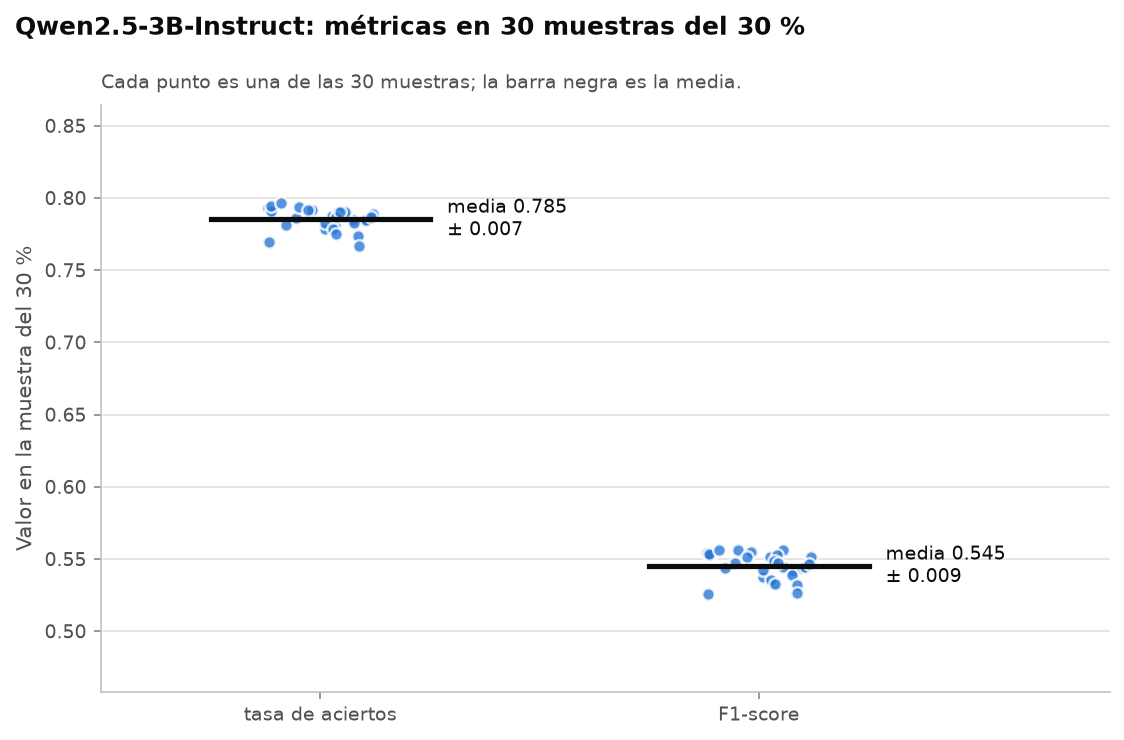
\includegraphics[width=\linewidth]{qwen2-5-3b-instruct-metricas-en-30-muestras-del-30.png}
\caption{Variación entre muestras de las predicciones fijas de Qwen; no
representa variación entre entrenamientos del modelo.}
\end{figure}

\paragraph{Errores y alcance.} Sobre todo el dataset, Qwen detectó 717 de
747 spam (recobrado 96.0\,\%), pero marcó como spam 1168 de los 4827 ham
(24.2\,\%). La precisión de spam fue 38.0\,\%: predijo 1885 spam, de los
cuales solo 717 eran correctos. En las muestras hubo, en promedio, 349.9
falsos positivos y 9.0 falsos negativos. El F1 bajo se explica principalmente
por las falsas alarmas, no por respuestas ambiguas. Incluso la tasa de
aciertos queda por debajo de predecir siempre ham (86.6\,\% en el dataset),
aunque esa regla trivial tendría F1 cero para spam.

\begin{figure}[H]
\centering
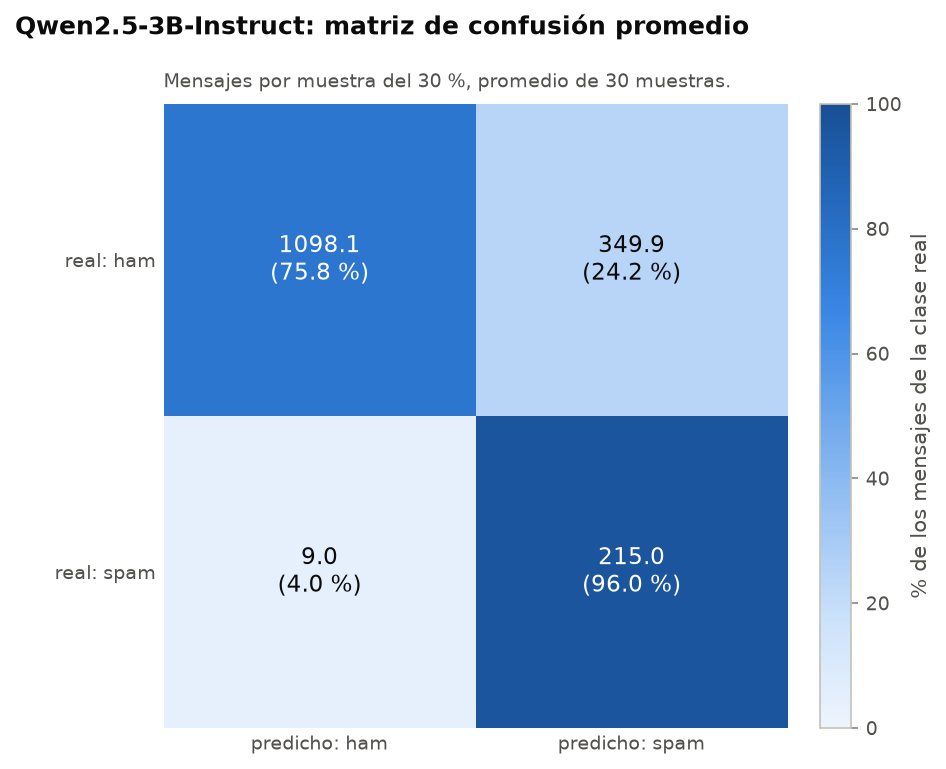
\includegraphics[width=0.86\linewidth]{qwen2-5-3b-instruct-matriz-de-confusion-promedio.png}
\caption{Confusión promedio de Qwen. La abundancia de ham marcado como spam
limita la precisión a pesar de detectar la mayor parte del spam.}
\end{figure}

Este resultado corresponde al modelo, prompt sin ejemplos y decodificación
confirmados. No se cambió el prompt después de observar las métricas.
Tampoco permite concluir que cualquier LLM sea inferior: evalúa esta
configuración concreta. Quedan pendientes los dos modelos adicionales de
3.2, si el equipo decide realizar el extra.

\subsection{Ajuste fino eficiente}

TODO (punto 3.3, extra): describir el ajuste con LoRA \cite{hu2021lora} o
DoRA \cite{liu2024dora} y analizar sus resultados.

\section{Pruebas unitarias}
\label{sec:pruebas}

El enunciado exige al menos dos pruebas unitarias para \texttt{forward} y
dos para \texttt{train\_logistic\_regression}. Las pruebas están en
\texttt{tests/test\_punto1.py} y se ejecutan en la sección ``Pruebas
unitarias'' del notebook y con \texttt{pytest}.

\subsection{Evaluación del modelo}

TODO (punto 1.1a): describir cada prueba de \texttt{forward} y qué verifica.

\subsection{Entrenamiento}

TODO (punto 1.2a): describir cada prueba del entrenamiento y qué verifica.

\section{Comparación de resultados}
\label{sec:comparacion}

TODO: comparar todos los métodos con la tabla y los diagramas de caja de la
sección ``Comparación de resultados'' del notebook.

\section{Conclusiones}
\label{sec:conclusiones}

\begin{itemize}
    \item La regresión logística implementada en PyTorch, con evaluación,
    gradiente y entrenamiento propios, separa sin error los datos
    sintéticos y alcanza sobre las características de MPNet una tasa de
    aciertos de $0.9906\pm0.0016$ y un F1 de $0.9641\pm0.0063$ en 30
    particiones. Es el método más sólido evaluado con 30 corridas.
    \item Reducir las 768 características a 384 componentes principales
    conserva el 96.16~\% de la varianza y prácticamente el mismo F1
    ($-0.0004$ en promedio). Con 2 componentes se pierde información útil
    para separar las clases y el F1 baja a 0.7845.
    \item El detector de anomalías por histogramas funciona sin ejemplos de
    spam, pero queda por debajo de la regresión en las 30 particiones (F1
    $0.7043\pm0.0247$ con $D=2$). Su punto débil son los ham poco
    frecuentes que marca como spam. Además, la suma de verosimilitudes de
    muchas componentes favorece al spam: con $D=384$ el detector casi no lo
    encuentra.
    \item Los modelos de lenguaje sin ajuste reconocen casi todo el spam,
    pero producen muchas falsas alarmas; el mayor modelo evaluado, Qwen 14B
    en NF4, obtiene el mejor F1 de los tres (0.7126).
    \item Un ajuste eficiente con LoRA sobre Qwen 14B en NF4 corrige ese
    sesgo: en su prueba reservada, los falsos positivos bajan de 174 a 5 y
    el F1 sube de 0.7120 a 0.9708, también en las filas cuyo texto no
    aparece en el entrenamiento.
    \item La tasa de aciertos sola es engañosa en este dataset desbalanceado:
    predecir siempre ham ya da 0.866. El F1 de la clase spam distingue
    mejor los métodos y refleja el costo de las falsas alarmas.
\end{itemize}

\subsection{Limitaciones}
\label{sec:limitaciones}

\begin{itemize}
    \item Las 30 particiones y las 30 muestras se toman del mismo dataset y
    se solapan; sus desviaciones describen la variación entre particiones,
    no intervalos de confianza de experimentos independientes.
    \item La partición es por filas y conserva los textos repetidos del
    archivo original. En promedio, el 9.7~\% de los mensajes de prueba
    (entre 145 y 181 de 1672) tiene una copia en el entrenamiento, lo que
    puede sobreestimar el desempeño en mensajes nuevos.
    \item El detector usa $D=2$, elegida con validación interna, en lugar
    de reutilizar $D=384$ como pide la lectura literal del apartado 2.1.
    Ambos casos se informan, y la elección de $D$ usó etiquetas de spam de
    validación, por lo que el procedimiento completo no es enteramente no
    supervisado.
    \item Los modelos de lenguaje sin ajuste y el modelo ajustado se evalúan
    con protocolos distintos de los puntos 1 y 2. El ajuste con LoRA es un
    único entrenamiento en una partición, sin estimación de su variabilidad.
    \item No se comprobó si los corpus de preentrenamiento de los modelos de
    lenguaje incluyen esta colección pública, así que no puede descartarse
    exposición previa a los mensajes.
    \item Las comparaciones entre modelos de lenguaje cambian a la vez
    familia, tamaño y precisión de los pesos; no aíslan el efecto de cada
    factor.
\end{itemize}


\bibliographystyle{plain}
\bibliography{references}

\end{document}
